In this chapter, we discuss the Second Law of Thermodynamics, and how it ties to entropy, which is the final property we will discuss in this book.  The Second Law helps us determine which processes are possible, and does so through entropy balance.  We will start with a brief discussion of entropy.

%--------------------------------------------------------------------
\section{Entropy}
%--------------------------------------------------------------------

Entropy is a property that is typically associated with the disorder of a system.  In other words, when a system is perfectly ordered (crystalline structure, with no atoms out of place), entropy will be at a minimum.  Disorder for a system means that it is hard to tell where an atom or molecule is at any particular point in time.  Figure \ref{fig:molecularEntropy} shows the relative level of disorder for solids, liquids, and gases.

\begin{figure}[H]
\centering
\begin{subfigure}{.3\textwidth}
  \centering
  \includegraphics[width=.9\linewidth]{molecularSolid}
  \caption{In many solids, atoms can vibrate, but rarely change position in their lattice structure.}
  \label{fig:molecularSolid}
\end{subfigure}\hfill
\begin{subfigure}{.3\textwidth}
  \centering
  \includegraphics[width=.9\linewidth]{molecularLiquid}
  \caption{In liquids, molecules are able to move relative to one another, but are closely confined.}
  \label{fig:molecularLiquid}
\end{subfigure}\hfill
\begin{subfigure}{.3\textwidth}
  \centering
  \includegraphics[width=.9\linewidth]{molecularGas}
  \caption{In gases, molecules are able to move freely, only occasionally colliding with other molecules.}
  \label{fig:molecularGas}
\end{subfigure}
\caption{Entropy is related to the amount of disorder in a system, which varies significantly between solids, liquids, and gases.}
\label{fig:molecularEntropy}
\end{figure}

For solids, atoms are mostly constrained, though there will be some vibration as temperature increases.  This means that there are relatively few options for an atoms location, and thus, minimal disorder.  For liquids, molecules are able to move somewhat freely, but are generally packed closely together with other molecules, which leads to significantly more entropy than for solids.  For gases, molecules are even more free to move than in liquids, with only occasional collisions with other molecules.  Thus, we assume that gases will have more disorder (and more entropy) than either liquids or solids.

\subsection{Entropy as a Property}
%--------------------------------------------------------------------

In addition to the difference between phases, we also know that temperature leads to an increase of the average movement of molecules within a substance.  An increase in temperature, therefore, can be assumed to increase the level of entropy.

Likewise, more volume available for a substance to spread out in leads to more locations for a given molecule to be at a given time.  So larger specific volume is also associated with higher entropy.  Figure \ref{fig:EntropyTv} is a contour plot of entropy on the $T$-$v$ diagram for water.

\begin{figure}[H]
  \centering
  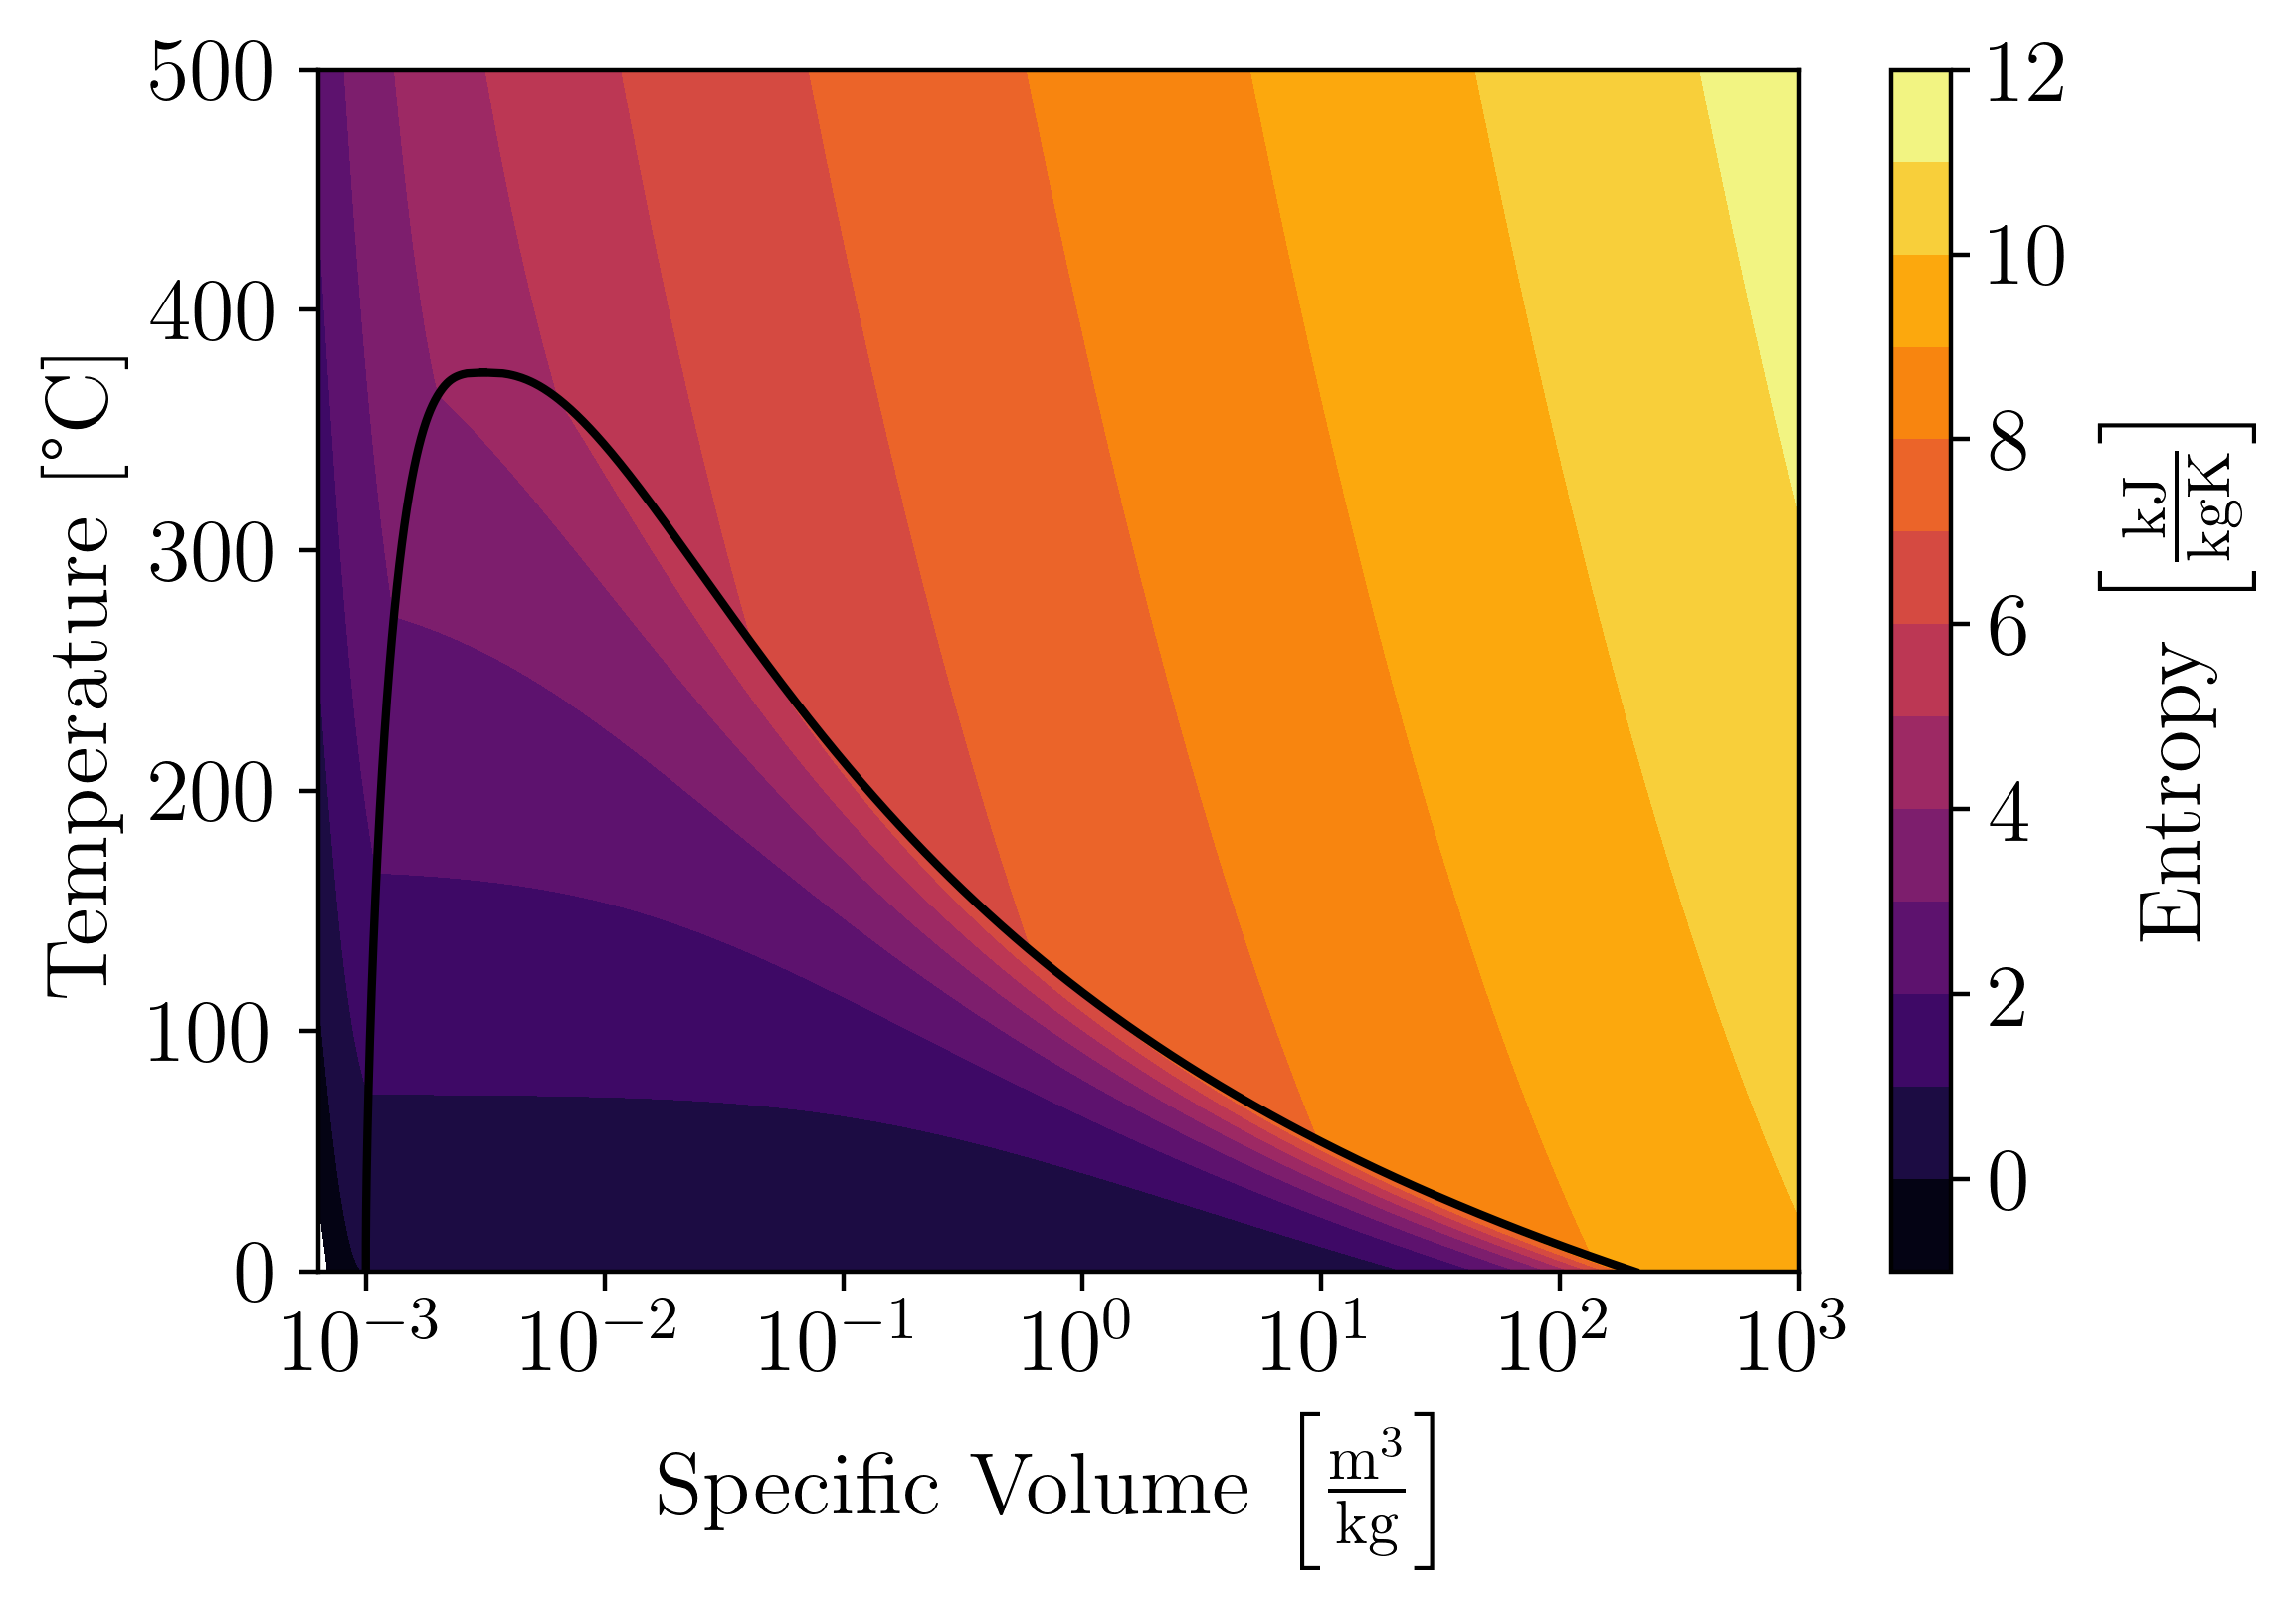
\includegraphics[width=.8\linewidth]{EntropyTv}
  \caption{A contour plot of entropy overlaid on the vapor curve in the $T$-$v$ diagram.}
  \label{fig:EntropyTv}
\end{figure}%

Finally, thinking of the ideal gas law, higher pressure will lead to lower specific volume for a given temperature, so we typically associate higher pressure with lower entropy.

\subsection{Entropy in Statistical Mechanics}
%--------------------------------------------------------------------

There is a way to determine the entropy by considering the number of {\bf microstates} that could make up a given state.  A microstate is a specific arrangement of molecules, including their position, velocity, vibration, and rotation.  States with more entropy could be generated through a greater number of microstates.  Entropy is defined as follows:
\begin{equation}\label{eq:Boltzmann}
  S = k_B \log \Omega
\end{equation}
In Equation \ref{eq:Boltzmann}, $S$ is the entropy of the system in $\frac{\rm kJ}{\rm K}$, $k_B$ is the Boltzmann constant: $1.381\times 10^{-26}\frac{\rm kJ}{\rm K}$, and $\Omega$ is the number of microstates for a given volume, number of atoms, and internal energy of the state.

Note that if only a single arrangement of molecules could define a state, the entropy would be exactly zero.  This occurs for molecules in crystalline solids (restricting their position) with zero energy (restricting their movement).  However, for common use, a reference value is typically chosen to be a zero point.  In this book, for instance, the triple point of water is given both an internal energy and entropy of zero, even though it could be cooled below that point.  In other words, if you see a negative entropy value, it means that it is less than a reference point, not negative in a true sense.

%The details of statistical mechanics are far beyond the scope of this book, so for our analysis, we will treat entropy as simply another tool in our toolbox.

%--------------------------------------------------------------------
\section{Reversibility} \label{sec:reversibility}
%--------------------------------------------------------------------

Entropy plays a central role as we consider {\bf ideal} processes.  Specifically, entropy is {\bf generated} any time we have a non-ideal process.  Non-ideal processes occur primarily because of friction, but can also occur when we violate the {\bf quasi-equilibrium} assumption that we discussed back in Section \ref{sec:states}.

\subsection{Friction}
%--------------------------------------------------------------------

Consider a block being pushed up a hill.  In the idealized case (no friction between the block and the hill), all of the work done is transferred to potential energy.  We could theoretically return down the hill, letting the block push us instead, and the net amount of work would be exactly zero.  This situation, where we can return to an initial state with no net loss is a {\bf reversible} process.

In a more real scenario, we could consider friction between the block and the hill.  In this situation, some fraction of our work will be used to overcome friction.  The potential energy at the top of the hill will be less than the amount of work we used to push the block.  If we tried to extract our work this time, we would start at a deficit, and then lose even more as friction stole energy on the way down!  This more realistic situation is an example of an {\bf irreversible} process.

Thinking about the First Law of Thermodynamics, it may seem like the irreversible process above violates the conservation of energy.  However, friction takes mechanical energy and transforms it into thermal energy.  After pushing the block and returning to the bottom, we have lost some amount of work, but the block has gained an equivalent amount of heat.

\subsection{Non-equilibrium Processes}
%--------------------------------------------------------------------
Another possibility of wasting work can occur when we perform a process too quickly.  Consider the piston undergoing compression shown in Figure \ref{fig:reversibility}.  Pressure does not change instantaneously.  In fact, any movement of the piston will create a wave in the volume which moves at the speed of sound.

\begin{figure}[H]
  \centering
  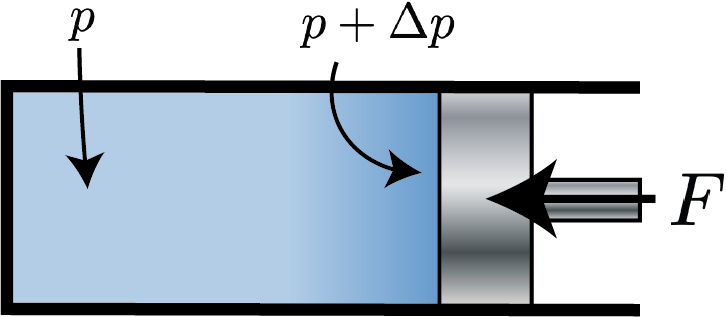
\includegraphics[width=.75\linewidth]{NonEquilibrium}
  \caption{A piston undergoing high-speed compression experiences higher pressure close to the piston.}
  \label{fig:reversibility}
\end{figure}

If the piston continues to compress before the pressure wave travels through the volume, it will push on air that has a higher pressure than the average within the volume.  Higher pressure means more work, but eventually, the pressure will even out. In the end, there will be no additional compression because of the higher work.  Instead, that additional energy will be transformed into heat.

Likewise, in an expansion process, if the pressure is not given a chance to equilibrate, it will be lower near the piston, meaning that less work will be extracted than expected.  Once again, the energy that was not extracted will be converted into heat.

Thus, in both types of irreversibility, we see that the final effect is to lose some amount of mechanical energy (work), with a commensurate increase in the internal energy (heat) of our system.

\subsection{Reversibility and Entropy} \label{sec:reversibilityEntropy}
%--------------------------------------------------------------------
We stated above that entropy was generated for non-ideal, or irreversible processes.  Based off the generation of heat for both types of irreversible processes above, we can guess that there will also be a change of entropy whenever heat is transferred in or out of a system.

However, when a process is reversible and no heat is transferred, there will be no change in entropy.  Recall our discussion of adiabatic processes in Section \ref{sec:ch3_idealGasAdiabatic}, in which we teased the term {\bf isentropic relations}.  In fact, there is an additional requirement to use those equations: the processes must be reversible.  Any friction or non-equilibrium effects will lead to conversion of work energy to heat energy, breaking the validity of the equations.

For isentropic (adiabatic and reversible) processes in steam or R134a, we can instead use the steam tables or CoolProp, assuming that $\Delta s = 0$.

For adiabatic and irreversible processes, we know that entropy will be generated.  This means that $\Delta s > 0$.  There cannot be an adiabatic process in which entropy is reduced.  In order to reduce entropy within a system, we must transfer it out of the system.  That will be the subject of Section \ref{sec:entropyTransfer}.

One final note: there is no real process that is also reversible.  In fact, we often use the word {\bf ideal} to mean reversible and {\bf real} to mean irreversible.  

% -------------------------------------------------------------------
\section{Entropy Transfer} \label{sec:entropyTransfer}
% -------------------------------------------------------------------
We saw in Section \ref{sec:reversibility} that entropy was related to heat energy.  In fact, heat transfer is the only way to transfer entropy into or out of a system.

\subsection{Entropy Transfer in Statistical Mechanics}
%--------------------------------------------------------------------
From a molecular point of view, the only ``true'' properties are the internal energy (how fast are the molecules moving, vibrating, or spinning on average), entropy (how many microstates are possible for a given macrostate), and specific volume (how much volume do these molecules inhabit).  With this context, we can return to an analysis similar to Section \ref{sec:specificHeats}:
\begin{align*}
  u &= u(s, v) \\
  du &= \frac{\partial u}{\partial s}ds + \frac{\partial u}{\partial v}dv \\
  du &= \left[\frac{d u}{d s}\right]_v ds + \left[\frac{d u}{d v}\right]_s dv
\end{align*}

Let us first think of an isentropic situation, and set $ds = 0$.  In this case, we get:
\begin{equation*}
  du = \left[\frac{d u}{d v}\right]_s dv
\end{equation*}
Now we are left to ask what sorts of situations can change the internal energy without changing entropy.  Because entropy is so closely related to heat transfer, we will assume that any heat transfer will cause a change in entropy.  Energy transfer through work is the only other option.  Knowing that $\delta w = p dv$ and $du = \delta q - \delta w$ leads us to the following realization:
\begin{equation} \label{eq:statMechPressure}
  \left[\frac{d u}{d v}\right]_s = -p
\end{equation}
Pressure emerges as a property that defines how the internal energy changes as volume changes.

Now, for constant volume, we know that heat transfer is the only way to affect the internal energy.
\begin{equation*}
  du = \delta q = \left[\frac{d u}{d s}\right]_v ds
\end{equation*}
Although we will not prove it here, this derivative is actually temperature:
\begin{equation} \label{eq:statMechPressure}
  \left[\frac{d u}{d s}\right]_v = T
\end{equation}
Like pressure, temperature emerges out of this molecular understanding of matter.  The end result of this exercise is a new form of the First Law of Thermodynamics, based solely on properties and their changes:
\begin{equation} \label{eq:FirstLawRevisited}
  du = T\,ds - p\,dv
\end{equation}

Finally, let's define the mechanism of entropy transfer:
\begin{equation} \label{eq:Tds}
  ds = \frac{\partial q}{T}
\end{equation}
Equation \ref{eq:Tds} states that heat transfer naturally yields a change in entropy, with heat transfer into a system causing an increase of entropy.
Additionally, more heat transfer is required at higher temperature to cause a change in entropy.  At low temperatures, less heat transfer is required to result in a large change in entropy.

\subsection{Defining Entropy for an Ideal Gas}
% -------------------------------------------------------------------

For ideal gases, we can go further in our analysis.  Taking the ideal gas law ($pv = RT$) in conjunction with Equation \ref{eq:FirstLawRevisited} allow us to write:
\begin{equation} \label{eq:idealEntropy1}
  ds  = \frac{du}{T}+ \frac{pdv}{T} \quad\rightarrow\quad ds = c_v \frac{dT}{T} + R\frac{dv}{v}
\end{equation}
Integrating \label{eq:idealEntropy1} (and assuming that $c_v$ is constant) results in:
\begin{align} 
  \nonumber  \int ds &= c_v \int \frac{dT}{T} + R \int \frac{dv}{v} \\
  \label{eq:idealEntropy2} s_2 - s_1 &= c_v \ln \left(\frac{T_2}{T_1}\right) + R \ln \left(\frac{v_2}{v_1}\right)
\end{align}

Alternatively, we can look back at the definition of enthalpy in Equation \ref{eq:dhExpanded} and replace $du$ in Equation \ref{eq:FirstLawRevisited} as follows:
\begin{equation*}
  dh - p\,dv - v\,dp = T\,ds - p\,dv
\end{equation*}
Following the same steps that led to Equation \ref{eq:idealEntropy2}:
\begin{align}
  \nonumber ds  &= \frac{dh}{T}- \frac{vdp}{T} \quad \rightarrow\quad ds = c_p \frac{dT}{T} + R\frac{dv}{v} \\
  \nonumber  \int ds &= c_p \int \frac{dT}{T} - R \int \frac{dp}{p} \\
  \label{eq:idealEntropy3} s_2 - s_1 &= c_p \ln \left(\frac{T_2}{T_1}\right) - R \ln \left(\frac{p_2}{p_1}\right)
\end{align}

Equations \ref{eq:idealEntropy2} and \ref{eq:idealEntropy3} describe the change of entropy in an ideal gas.

\begin{quoteWithTitle}{Change of Entropy in an Ideal Gas}%
  \begin{equation*}
    s_2 - s_1 = c_v \ln \left(\frac{T_2}{T_1}\right) + R \ln \left(\frac{v_2}{v_1}\right) =
    c_p \ln \left(\frac{T_2}{T_1}\right) - R \ln \left(\frac{p_2}{p_1}\right)
  \end{equation*}
\end{quoteWithTitle}

These equations can also be used to produce the adiabatic relations we derived in Section \ref{sec:ch3_idealGasAdiabatic} by setting the change in entropy ($s_2 -s_1$) equal to zero.

\subsection{Entropy for Liquids and Solids}
%--------------------------------------------------------------------
For liquids and solids, we can again use Equation \ref{eq:FirstLawRevisited}, recognizing that $dv$ is zero for incompressible materials:

\begin{equation*}
  du = Tds - p\cancelto{0}{dv} \quad\rightarrow\quad ds = \frac{du}{T}
\end{equation*}

Assuming that the specific heat is a constant $c$, we can integrate as follows:
\begin{equation} \label{eq:entropyChangeIncompressible}
  \int ds = c\int\frac{dT}{T} \quad\rightarrow\quad s_2 - s_1 = c \ln \left(
 \frac{T_2}{T_1}\right)
\end{equation}

Therefore, entropy is defined purely by the temperature change for solids and liquids.

\subsection{Additional Thoughts on Pressure and Temperature}
% -------------------------------------------------------------------
Consider a piston between two cavities, as shown in Figure \ref{fig:doublePistonWork}.  Each cavity is at a different pressure, the net effect of which is to cause a force on the piston.  Assuming a frictionless environment, the piston will move until the pressure is balanced on both sides.
\begin{figure}[H]
\centering
\begin{subfigure}{.45\textwidth}
  \centering
  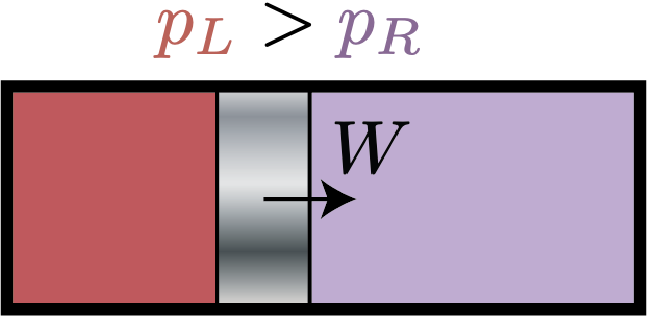
\includegraphics[width=.6\linewidth]{PressureBalance}
  \caption{The difference in pressure will cause work on the piston until pressure is balanced between the two cavities.}
  \label{fig:doublePistonWork}
\end{subfigure}%
\hfill
\begin{subfigure}{.45\textwidth}
  \centering
  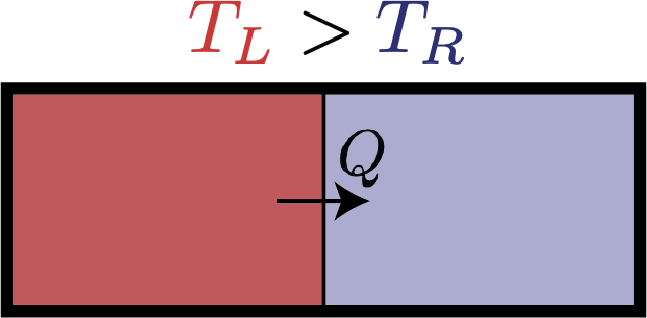
\includegraphics[width=.6\linewidth]{TemperatureBalance}
  \caption{The difference in temperature will cause heat transfer until temperature is balanced between the two cavities.}
  \label{fig:doubleCavityHeatTransfer}
\end{subfigure}
\caption{Work and heat transfer cause pressure and temperature to tend toward balance.}
\label{fig:statMechPressureAndTemp}
\end{figure}
Likewise, looking at Figure \ref{fig:doubleCavityHeatTransfer}, the difference in temperature across the two cavities leads to heat transfer across the boundary.  Heat will continue to flow until the temperature is balanced on both sides.  This process will transfer entropy from left to right, and also increase the total amount of entropy.  This process is investigated in Example \ref{ex:entropyMaximization}.

\begin{example}[label=ex:entropyMaximization]{Maximizing Entropy Through Heat Transfer}
  A thin barrier separates equal masses of water such that each side has a volume of 10 L and a mass of 0.1 kg.  The walls are insulated, meaning that no heat can escape.  On the left, the steam is at 300°C, and on the right, the steam is at 200°C.  Find the resting state of the steam, and evaluate the amount of entropy change in the system.

  \begin{enumerate}[a)]
  \item Find the entropy on each side prior to heat transfer, as well as the total amount of entropy in the system.
  \item Find the temperature of the final system.
  \item Find the entropy on each side after heat transfer, as well as the total amount of entropy in the system.
  \item How much did entropy change on each side?  How much did the total entropy change?
  \end{enumerate}
  \subsubsection*{Entropy Before Heat Transfer}
  The entropy prior to heat transfer can be determined from the steam tables.
  Each side has the same specific volume, calculated as follows:
  \begin{equation*}
    v = \frac{V}{m} = \frac{0.01\ \rm m^3}{0.1\ \rm kg} = 0.1\ \frac{\rm m^3}{\rm kg}
  \end{equation*}

  Thus, the left side is superheated steam, with $s_{left}=6.651\ \frac{\rm kJ}{\rm kg\,K}$.  The right side is a mixture with a quality of 0.784, leading to an entropy of $s_{left}=5.545\ \frac{\rm kJ}{\rm kg\,K}$.

  We can find the total amount of entropy as follows:
  \begin{equation*}
    S_i = \sum_j m_js_j = 0.1\ {\rm kg} \left(6.651\ \frac{\rm kJ}{\rm kg\,K}\right) + 0.1\ {\rm kg} \left(5.545\ \frac{\rm kJ}{\rm kg\,K}\right) = \redbox{ 1.220 \ \frac{\rm kJ}{\rm K}}
  \end{equation*}
  
  \subsubsection*{Final Temperature}
  At the end of heat transfer, both states should have the same temperature.  Since both also have the same specific volume, they will share the same state exactly.

  This means that we can calculate the total internal energy of the system, divide it up between the two sides, and we will have our final state.

  \begin{equation*}
    U = \sum_j m_j u_j = 0.1\ {\rm kg} \left(2762.8\ \frac{\rm kJ}{\rm kg}\right) + 0.1\ {\rm kg} \left(2217.8\ \frac{\rm kJ}{\rm kg\,K}\right) =  498.06 \ \rm kJ
  \end{equation*}

  The final internal energy will be $u_f = U/\sum_i m_i$, or 498.06 kJ / 0.2 kg.  Thus, $u_f = 2490.3 \ \frac{\rm kJ}{\rm kg}$.

  We again go to the tables (or CoolProp) with $u$ and $v$ to find temperature: $\redbox{ T_f = 208.86°C }$.  This occurs as a mixture with a quality of 0.937.

  \subsubsection*{Final Entropy}
  We head to the tables one final time to find the final entropy: $\redbox{s_f = 6.116 \frac{\rm kJ}{\rm kg\,K}}$.

  Since this is the same for both sides, we can find the total entropy through $S_f = 0.2\ {\rm kg} s_f$.  Thus, $\redbox{S_f = 1.223 \ \frac{\rm kJ}{\rm K}}$.

  \subsubsection*{Change in Entropy}
  We can see that the specific entropy on the left side decreased from 6.651$\ \frac{\rm kJ}{\rm K}$ to 6.116$\ \frac{\rm kJ}{\rm K}$, while the specific entropy on the right side increased from 5.545$\ \frac{\rm kJ}{\rm K}$ to 6.116$\ \frac{\rm kJ}{\rm K}$.
  \begin{align*}
    \Delta s_L &= 6.116\ \frac{\rm kJ}{\rm kg\,K} - 6.651\ \frac{\rm kJ}{\rm kg\,K} = \redbox{-0.535\ \frac{\rm kJ}{\rm kg\,K}} \\
    \Delta s_L &= 6.116\ \frac{\rm kJ}{\rm kg\,K} - 5.545\ \frac{\rm kJ}{\rm kg\,K} = \redbox{0.571\ \frac{\rm kJ}{\rm kg\,K}} \\
    \Delta S &= 1.223\ \frac{\rm kJ}{\rm K} - 1.220 \ \frac{\rm kJ}{\rm K} = \redbox{0.003 \ \frac{\rm kJ}{\rm K}}
  \end{align*}

  Working through the example more accuracy gives a change of entropy of 3.474 $\frac{\rm J}{\rm K}$.

  \subsubsection*{Discussion}
  First off, through heat transfer, we were able to transfer entropy as well. The entropy of the left side decreased, while the entropy of the right side increased.  However, the act of transferring heat also increased the total entropy of the system.  Thus, unlike energy, it is possible to {\bf generate} entropy.  Additionally, the entropy of an isolated system (like the one in the example) will always be maximized when all components are at the same temperature.
\end{example}

Example \ref{ex:entropyMaximization} showed that heat transfer naturally led to entropy transfer between two systems.  Section \ref{sec:SecondLaw} investigates the byproduct of that heat transfer: the entropy generated by an irreversible process.

% -------------------------------------------------------------------
\section{Defining the Second Law} \label{sec:SecondLaw}
% -------------------------------------------------------------------
The simplest form of the Second Law is as follows:

\begin{quoteWithTitle}{The Second Law}{There can be no process or cycle in which entropy decreases globally.}
\end{quoteWithTitle}

We saw the possibility of an isentropic process in Section \ref{sec:reversibilityEntropy}.  However, for irreversible processes without heat transfer, entropy increased.  In Section \ref{sec:entropyTransfer}, we saw the possibility of {\bf locally} decreasing entropy, but always at the cost of increasing it elsewhere.  For any realistic heat transfer, there will always be a {\bf global} increase of entropy in the process.

Global, in this context, means considering the system that includes the surroundings.  For a simplified problem, that often just means including the hot and cold {\bf reservoirs} attached to the system.  Reservoirs are regions that have enough heat capacity to maintain a constant temperature even with the heat transfer associated with our system.

In addition to this simple form, we will investigate two other statements of the Second Law: the Clausius Statement and the Kelvin-Planck Statement.

\subsection{The Clausius Statement of the Second Law}
%--------------------------------------------------------------------
\begin{quoteWithTitle}{The Clausius Statement}{It is impossible to construct a device which operates on a cycle and produces no other effect than the transfer of heat from a cooler body to a hotter body.}
\end{quoteWithTitle}

To unpack that, let's first consider the ``transfer of heat'' part.  We saw in Example \ref{ex:entropyMaximization} that the natural flow of hot to cold increases global entropy.  It stands to reason that heat flow from cold to hot would instead decrease entropy, which violates the simple form of the First Law.

It may be obvious that heat transfer will not naturally happen in this manner, but the Clausius Statement forbids any device from completing this feat.  This situation is pictured on the left of Figure \ref{fig:clausiusViolator}.

\begin{figure}[H]
  \centering
  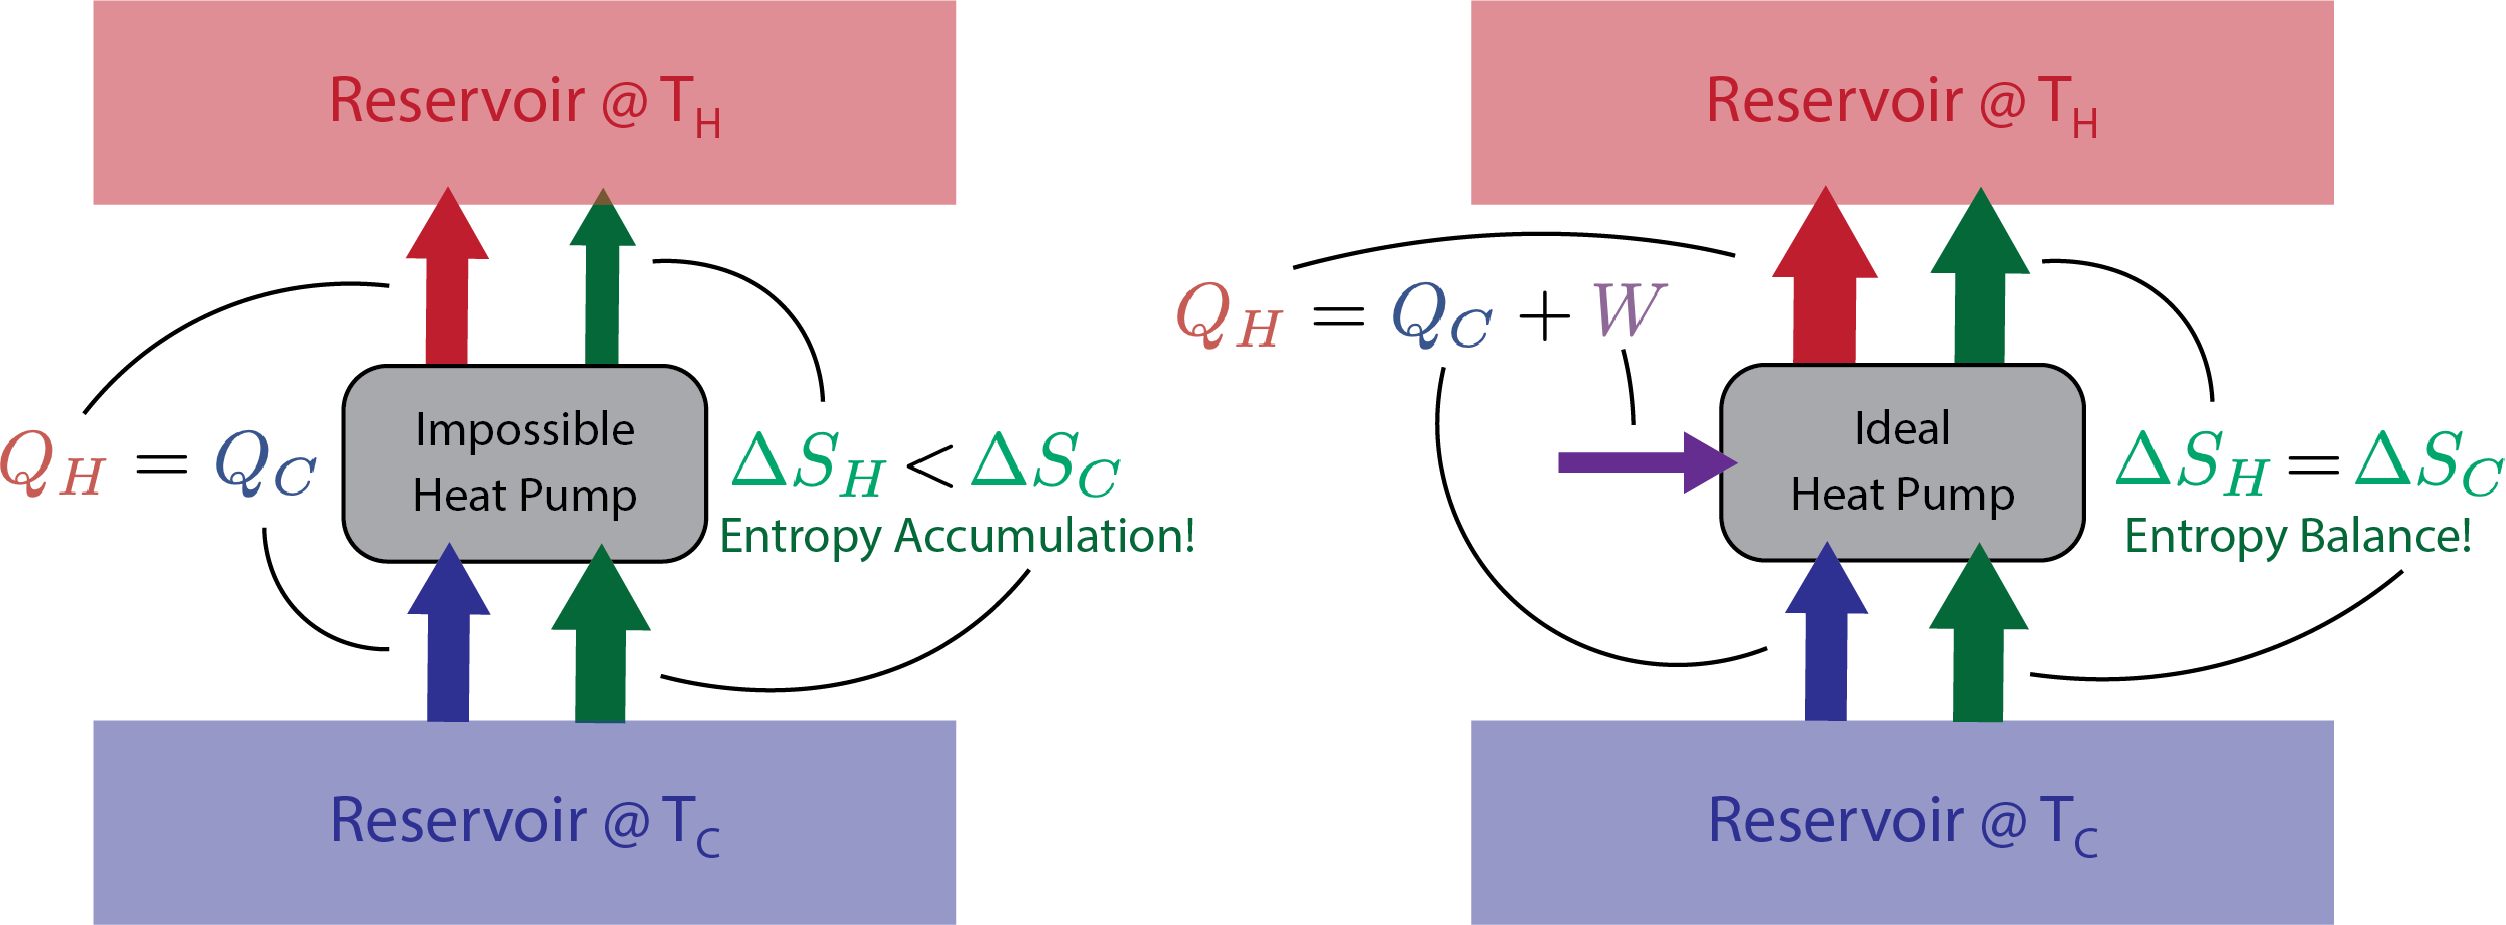
\includegraphics[width=.85\linewidth]{Clausius Statement}
  \caption{A visual depiction of a device outlawed by the Clausius statement of the Second Law beside an ideal device.}
  \label{fig:clausiusViolator}
\end{figure}

It can be seen that in the case where $Q_C = Q_H$, there is more entropy entering the heat pump than is leaving.  This is a direct result of Equation \ref{eq:Tds}: $ds = \frac{\delta q}{T}$.  In order to balance the entorpy transferred through $Q_C$ and $Q_H$, more heat transfer is needed at $T_H$ than at $T_C$.  To get that extra energy without changing the inflow of entropy, we must add work to the heat pump.  The corrected situation is shown on the right side of Figure \ref{fig:clausiusViolator}.

There is an exception implicitly mentioned in the Clausius Statement: devices that do not ``operate on a cycle''.  It is technically possible to remove heat from a cold body and add heat to a hot body without violating the Second Law.  However, the only way this is possible is by increasing the overall entropy inside the device.  If the entropy inside the device increased, there is no way for it to return to its original state {\bf without some other effect}, and therefore it cannot form a cycle.

Bottom Line: a cycle requires an influx of energy as work to move heat from cold to hot.

\subsection{Kelvin-Planck Statement of the Second Law}
%--------------------------------------------------------------------
There is an alternative statement of the Second Law, known as the {\bf Kelvin-Planck Statement}:

\begin{quoteWithTitle}{The Kelvin-Planck Statement}{It is impossible to construct a device which operates on a cycle and produces no other effect than the transfer of heat from a single body in order to produce work.}
\end{quoteWithTitle}

Thinking only about the First Law of Thermodynamics (energy conservation), there is nothing in the Kelvin-Planck Statement that seems impossible.  Energy enters a system as heat and leaves as work, thus maintaining a constant amount of energy in the system.

Unfortunately, when we consider entropy flow, we run into trouble.  Heat transfer into the system will always bring entropy with it.  Work leaving the system will either generate entropy (irreversible processes) or maintain a constant amount of it (reversible processes). Combining the two, we know that there will be a net gain of entropy in the system.  Once again, with a net gain of entropy, we cannot form a cycle.

The left side of Figure \ref{fig:kelvinPlanck} shows a device breaking the Kelvin-Planck statement by absorbing heat from a heat reservoir at $T_H$ and transforming that heat into work.  Note that entropy is also absorbed with the heat, but there is nowhere that entropy is rejected.
%
\begin{figure}[H]
  \centering
  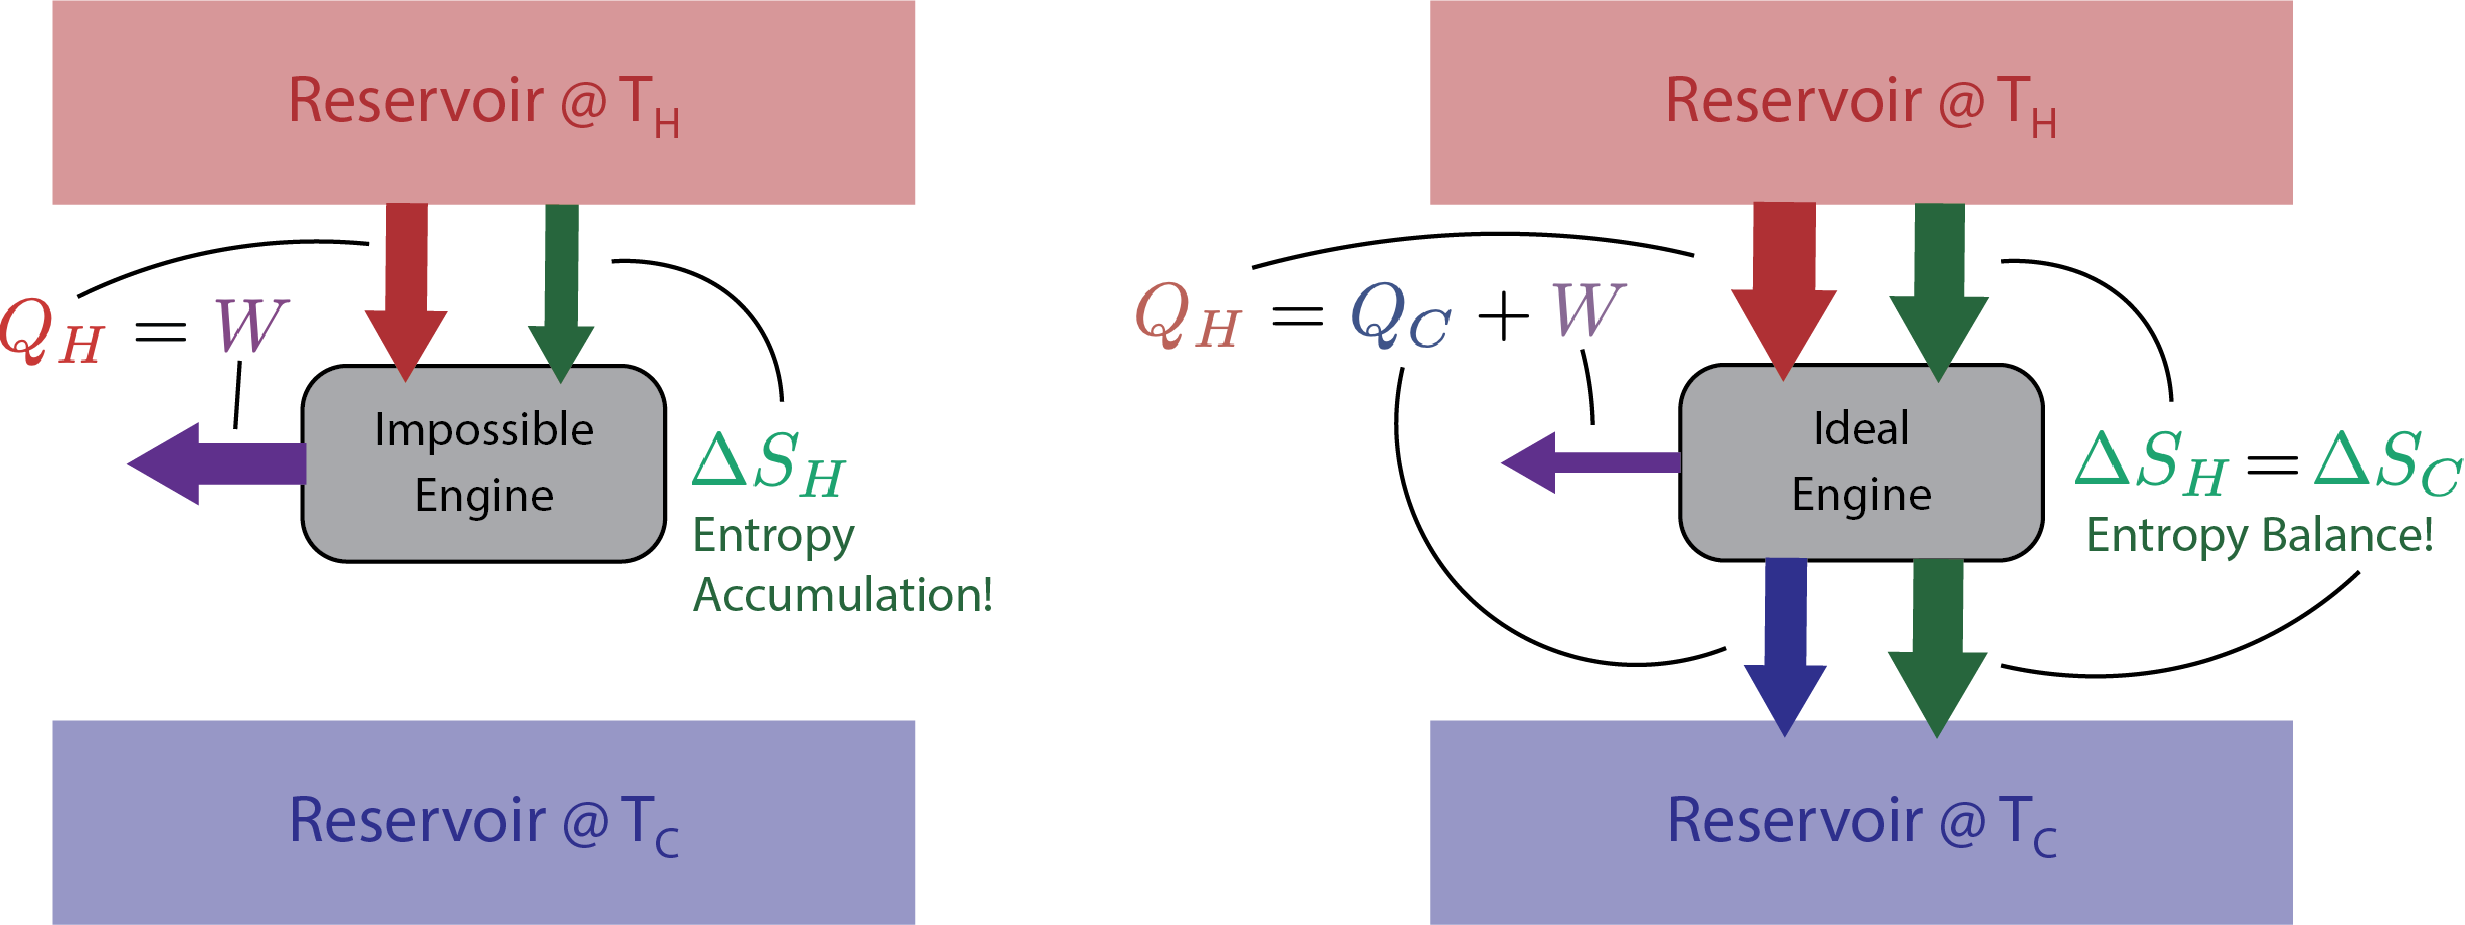
\includegraphics[width=.85\linewidth]{KP Statement}
  \caption{A visual depiction of a scenario outlawed by the Kelvin-Planck statement of the Second Law beside an ideal device.}
  \label{fig:kelvinPlanck}
\end{figure}%
%
The right side of Figure \ref{fig:kelvinPlanck} give the corrected picture.  In order to rid itself of excess entropy, the device must reject heat.

Bottom line: for a cycle to produce work, it must both accept and reject heat.

\subsection{Equivalence of Kelvin-Planck and Clausius Statements}
%--------------------------------------------------------------------
We showed above that the simple form of the Second Law implied both the Kelvin-Planck and Clausius Statements.  It should be no surpise, then, that we are able to show that both statements are equivalent.

First, let us consider the combination of cycles shown on the left side of \ref{fig:ClausiusEquivalence}.  First, we have a heat pump that violates the Clausius Statement, which we have labeled an ``impossible heat pump''.  Simultaneously, we run a perfectly legitimate engine.  The important thing to note here is that the heat transfer through the impossible heat pump perfectly matches the heat flow through the engine (the part not turned into work).

\begin{figure}[H]
  \centering
  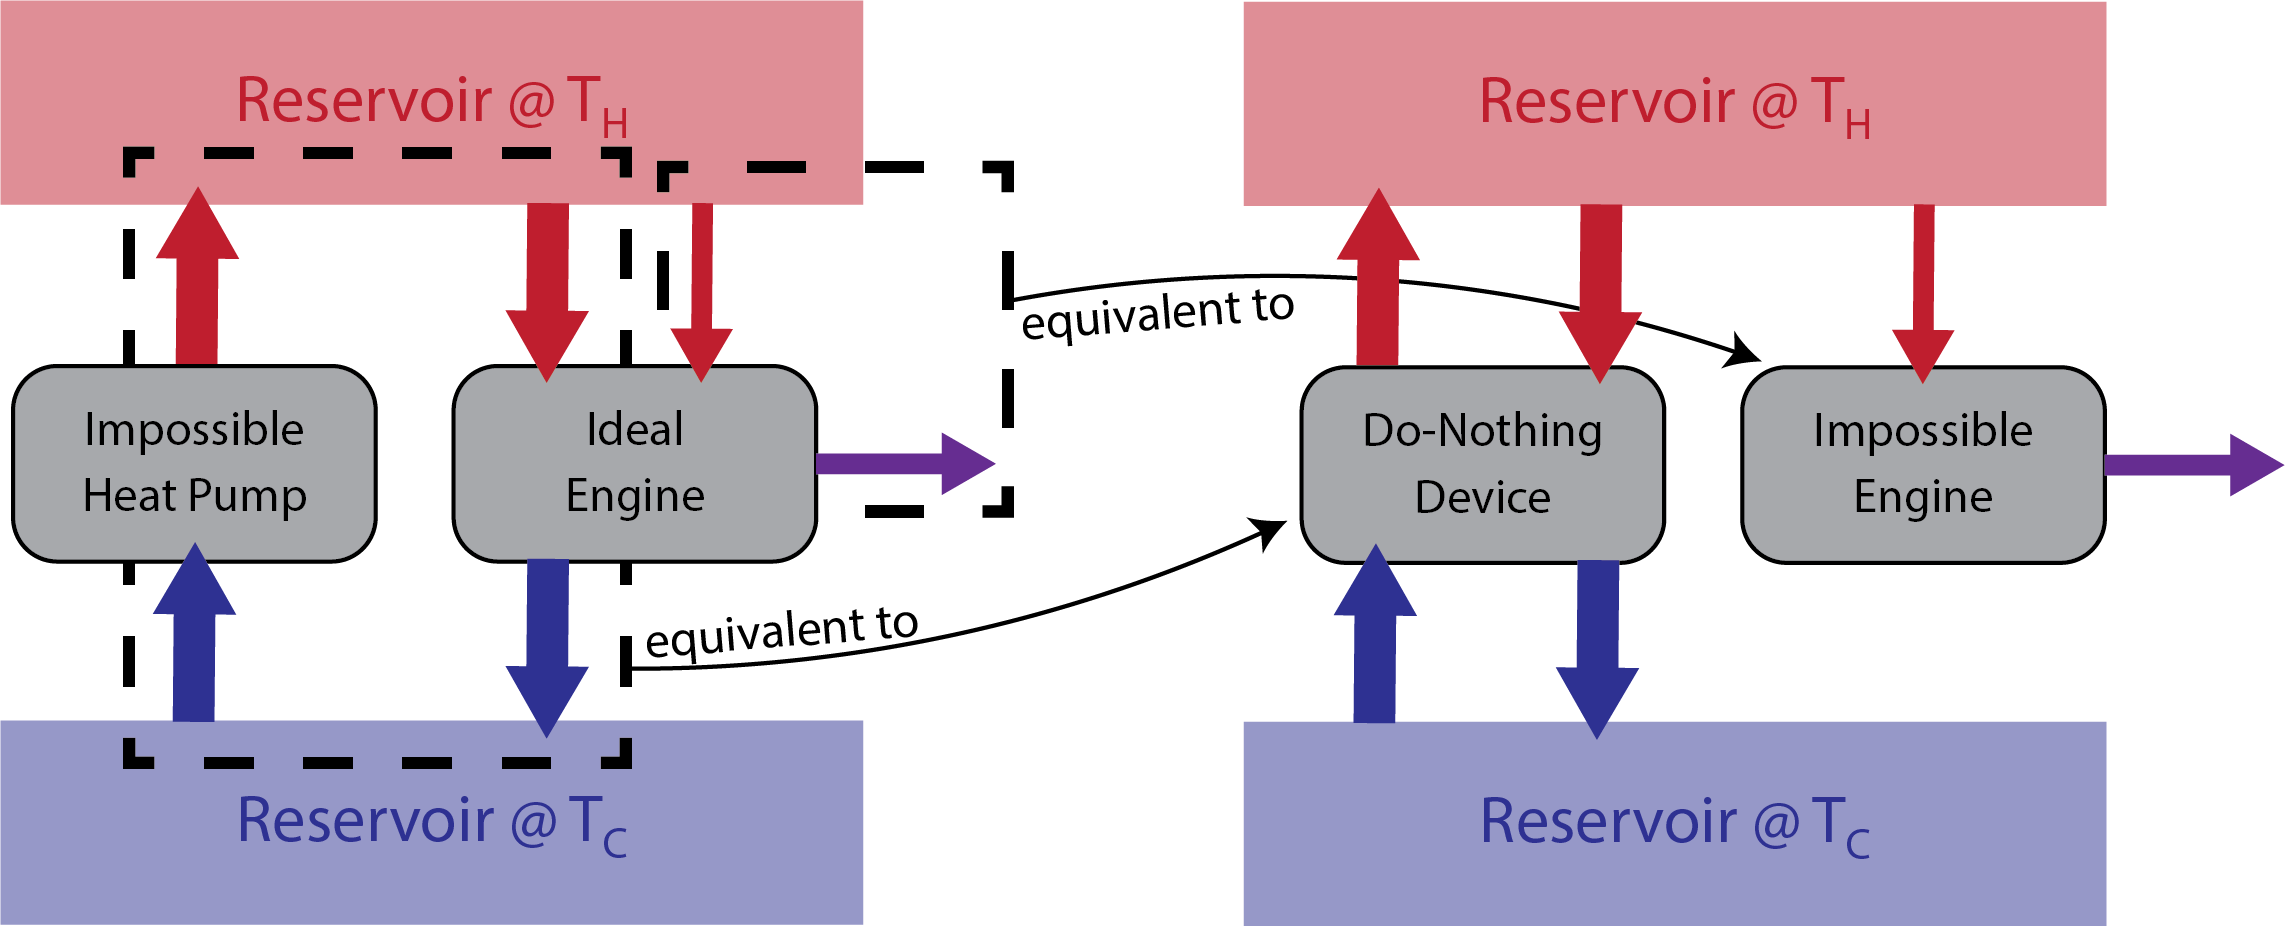
\includegraphics[width=.9\linewidth]{Clausius KP Equivalence}
  \caption{A heat pump in violation of the Clausius Statement paired with a perfectly legal heat engine.}
  \label{fig:ClausiusEquivalence}
\end{figure}

A different grouping of the heat flows allows us to see the violation of the Kelvin-Planck Statement.  Combining the illegal heat flow with the heat flow through the legitimate engine creates a device in which all the heat flows cancel: a ``do-nothing device''.  What remains is an ``impossible engine'', which converts heat directly into work.

Thus, each of our statements of the Second Law are functionally equivalent.

%--------------------------------------------------------------------
\section{Carnot Cycles and Ideal Efficiency}
%--------------------------------------------------------------------
The Carnot cycle is a primarily theoretical cycle that is intended to provide the maximum efficiency between two temperature reservoirs.

Heat transfer into the system occurs isothermally at the highest temperature possible, to minimize the entropy transferred into the system.  Likewise, heat transfer out of the system occurs at the lowest temperature possible, to maximize the entropy transferred out of the system.  Temperature change occurs adiabatically and isentropically.  Figure \ref{fig:carnotph} shows the cycle drawn on a $p$-$h$ diagram. %Figure \ref{fig:carnotEngine} shows the Carnot cycle in a closed system, while Figure \ref{fig:carnotph} shows the cycle in a $p$-$h$ diagram.

%\begin{figure}[H]
%  \centering
%  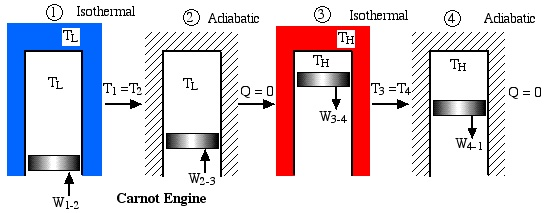
\includegraphics[width=.75\linewidth]{CarnotEngine}
%  \caption{The processes involved in the ideal Carnot Engine.}
%  \label{fig:carnotEngine}
%\end{figure}

\begin{figure}[H]
  \centering
  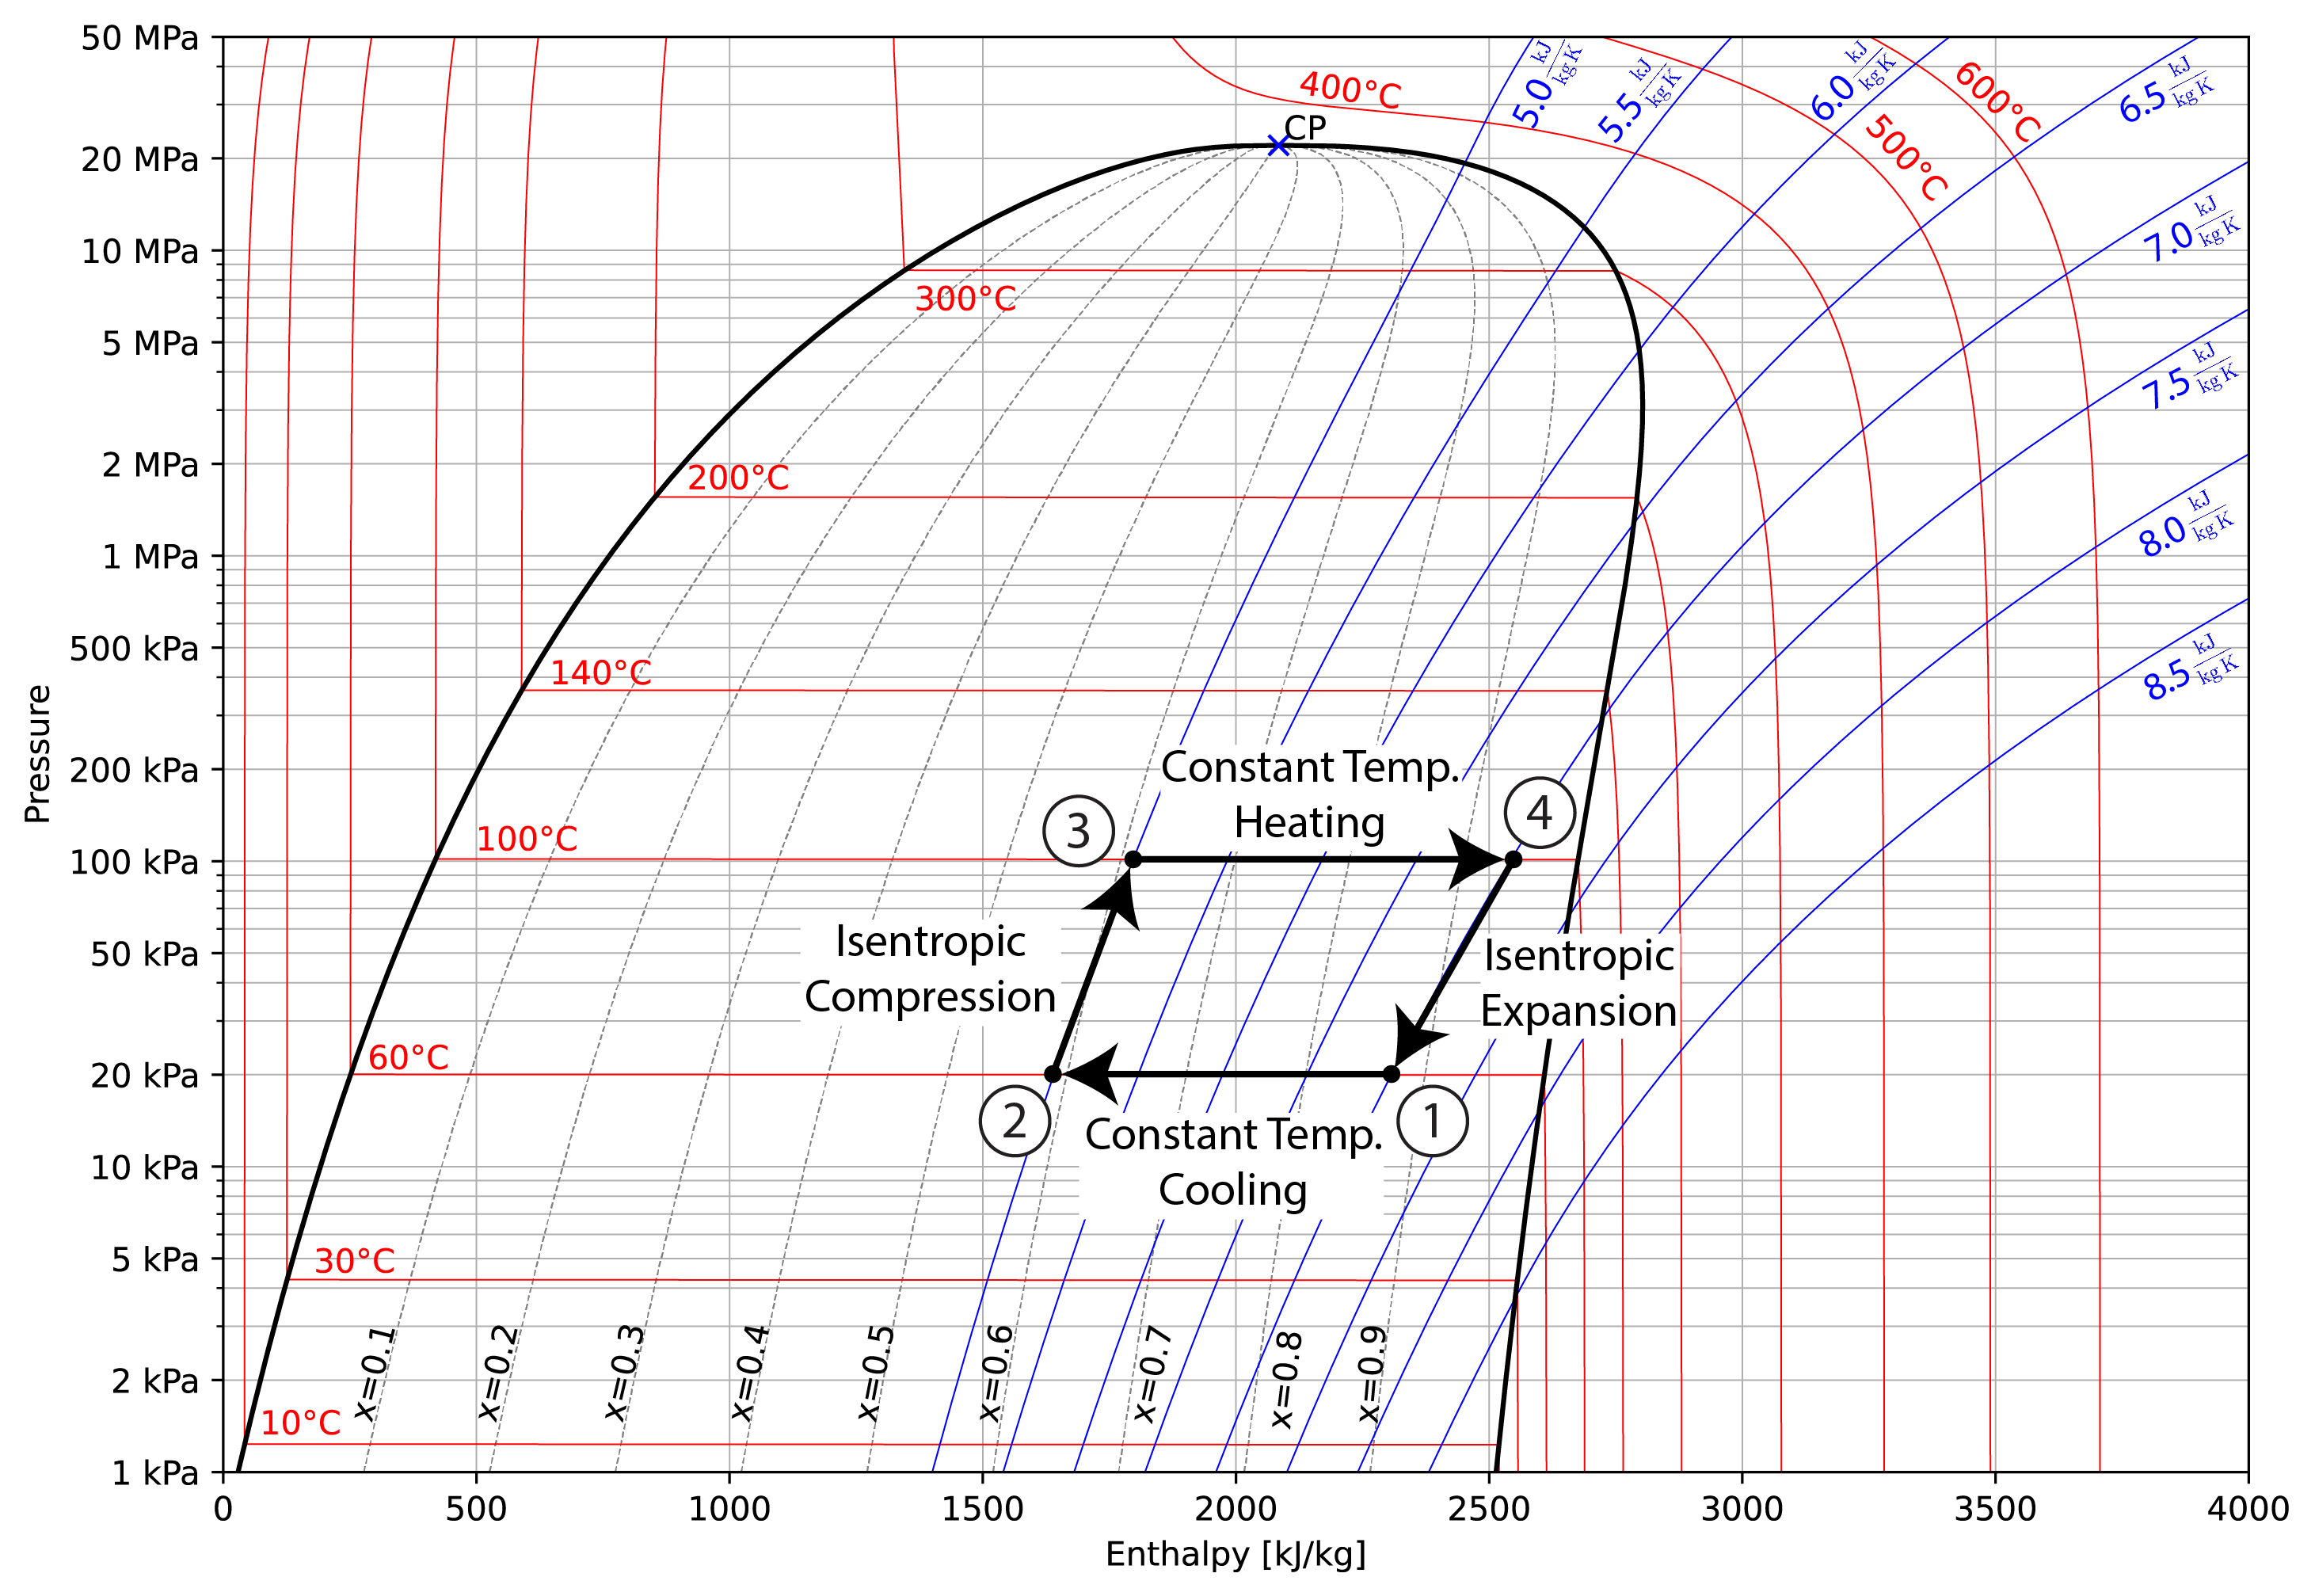
\includegraphics[width=.9\linewidth]{CarnotPH}
  \caption{A Carnot Cycle plotted on a $p$-$h$ diagram for steam.}
  \label{fig:carnotph}
\end{figure}

Note the frequent switching between constant temperature environments (necessitating ample heat flow) and adiabatic environments (requiring zero heat flow).  This change of environment is the primary problem with the Carnot cycle for practical purposes.

As you can see in Figure \ref{fig:carnotph}, the difference in entropy between states 1 and 2 perfectly matches the difference between states 3 and 4.  In other words, the entropy entering the system through $Q_H$ exits the system through $Q_C$.

\subsection{Carnot Cycle Analysis}
%--------------------------------------------------------------------
By setting the inflow of entropy equal to the outflow, we can determine the maximum possible difference between $Q_H$ and $Q_C$, which in turn will maximize work (recall that $W = Q_H - Q_C$).

\begin{align*}
  ds_{in} &= \frac{\delta q}{T_H} &  ds_{out} &= \frac{\delta q}{T_C}\\
  \Delta s_{in} &= \int \frac{\delta q}{T_H} = \frac{Q_H}{T_H}  &
  \Delta s_{out} &= \int \frac{\delta q}{T_C} = \frac{Q_C}{T_C} 
\end{align*}
This leads to a relationship between the heat transfers and the temperatures:
\begin{equation*}
 \Delta s_{in} = \Delta s_{out} \qquad \rightarrow \qquad \frac{Q_H}{T_H} = \frac{Q_C}{T_C}
\end{equation*}

We can rearrange this to build an equivalence between the heat transfer ratio and the temperature ratio for the Carnot cycle.
\begin{equation} \label{eq:QTequivalence}
  \frac{Q_C}{Q_H} = \frac{T_C}{T_H}
\end{equation}

Finally, let's revisit the equation for efficiency of an engine, letting $Q_{in}=Q_H$.
\begin{equation*}
  \eta_{th} = \frac{W_{net}}{Q_H} = \frac{Q_H - Q_C}{Q_H} = 1 - \frac{Q_C}{Q_H}
\end{equation*}
Using Equation \ref{eq:QTequivalence}, we can find the efficiency for a Carnot cycle based purely on the temperature of the reservoirs:
\begin{equation} \label{eq:CarnotEfficiency}
  \eta_{th, max} = 1 - \frac{T_C}{T_H}
\end{equation}

With a bit of work, we can also come up with the maximum theoretical coefficient of power for the refrigeration and heat pump cycles.

\begin{align}
  \label{eq:CarnotCOPR}  COP_{R, max}  &= \frac{T_C}{T_H - T_C} \\
  \label{eq:CarnotCOPHP} COP_{HP, max} &= \frac{T_H}{T_H - T_C} 
\end{align}

As always, the coefficient of performance for a heat pump will be exactly 1 larger than that for a refrigerator.

\begin{example}{Reversible Home Air Conditioner and Hot Water Heater}
  We wish to do a preliminary thermodynamic evaluation of the following proposed heat pump system designed for summertime hot water heating and space cooling.
  \begin{center}
    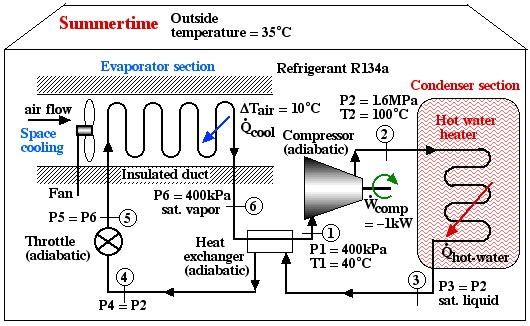
\includegraphics[width=0.7\textwidth]{ch5_P1}
  \end{center}

  Assuming that this system is required to maintain the home air at 20°C and the hot water at 50°C, we wish to determine the maximum possible theoretical Coefficients of Performance that could be obtained under these conditions.

  \begin{enumerate}[a)]
  \item Draw a diagram representing the heat pump system showing the flow of energy and source and sink temperatures.
  \item Determine the maximum possible Coefficient of Performance of a hot water heater ($COP_{HW}$) that could be obtained by a reversible heat pump.
  \item Determine the maximum possible Coefficient of Performance of a space cooling air conditioner ($COP_{AC}$) that could be obtained by a reversible heat pump.
  \item The actual Coefficients of Performance for the system shown above were found to be $COP_{HW} = 4.41$ and $COP_{AC} = 3.41$.  Compare those values to those of the reversible heat pump determine if the actual heat pump shown above is feasible. State the reasons for your conclusion.
  \end{enumerate}
  {\bf Solution:}
  For a), b), and c) we need to reduce the system complexity shown above to an energy flow diagram showing only the basic requirements - cool the air to 20°C and heat the water to 50°C. Given the temperature if the heat source (20°C) and the heat sink (50°C) we can evaluate the respective reversible Coefficients of Performance.

  \begin{center}
    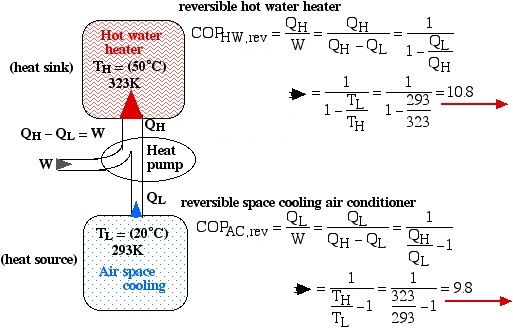
\includegraphics[width=0.7\textwidth]{rev_hotw_ac}
  \end{center}

  For question d) we use the accumulated knowledge that the conditions for thermal and mechanical reversibility are so difficult to realize that no practical heat pump or heat engine can attain more than 50\% to 60\% of the equivalent reversible (Carnot) performance. Thus comparing the actual to the reversible Coefficients of Performance we obtain:
  \begin{align*}
    \frac{COP_{HW, act}}{COP_{HW, rev}} &= \frac{4.4}{10.8} = 41\% \quad (<\ 50\%\quad \rightarrow \quad {\rm feasible!}) \\
    \frac{COP_{AC, act}}{COP_{AC, rev}} &= \frac{3.4}{9.8} = 35\% \quad (<\ 50\%\quad \rightarrow \quad {\rm feasible!})
  \end{align*}
  Both coefficients of performance were less than 50\% of their reversible values, meaning that they are indeed feasible.
\end{example}

\begin{homework}
  \question A heat pump is used to meet the heating requirements of a house and maintain it at 20°C. On a day when the outdoor air temperature drops to -10°C it is estimated that the house looses heat at the rate of 10 kW. Under these conditions the actual Coefficient of Performance ($COP_{HP}$) of the heat pump is 2.5.
  \begin{questionparts}
  \item Draw a diagram representing the heat pump system showing the flow of energy and the temperatures.
  \item Determine the actual power consumed by the heat pump \answer{[4 kW]}.
  \item Determine the power that would be consumed by a reversible heat pump under these conditions \answer{[1.02 kW]}.
  \item Determine the power that would be consumed by an electric resistance heater under these conditions \answer{[10 kW]}
  \item Determine if the performance of the actual heat pump is feasible.
  \end{questionparts}
  \question During an experiment conducted at 25°C, a student measured that a Stirling cycle refrigerator that draws 250W of power has removed 1000kJ of heat from the refrigerated space maintained at -30°C. The running time of the refrigerator during the experiment was 20 min.
  \begin{questionparts}
  \item Draw a diagram representing the refrigerator system showing the flow of energy and the temperatures.
  \item Determine the actual and reversible coefficients of performance \answer{[COPR = 3.33, COPR,rev = 4.42]}.
  \item Determine if these measurements are reasonable. \answer{[$COP_R/COP_{R,rev}$ = 75\% > 60\% - not feasible]}. State the reasons for your conclusions. 
  \end{questionparts}
\end{homework}

